\section{Results}
To understand how contributions by editors to articles shape the structure of collaboration in Wikipedia, we have performed a calibration of the bi-partite network random walker model on 12 Wikipedia categories (c.f. Table \ref{tab:statistics}) with 13 snapshots each (Figure \ref{fig:snapshots}). For each category and snapshot, we found the set of parameters $(\alpha^*,\beta^*)$, which maximize the fitness of the model to ground-truth metrics of article quality and editor expertise. Figure \ref{fig:landscape} shows typical optimization landscapes, which maximize the rank correlation $\rho_e$ (upper panel) between editor expertise $w_{e}$ obtained from the model and expertise obtained from state-of-the-art measures $\bar{w}_e$. The same is done for rank correlation $\rho_a$ between $w_a$ and $\bar{w}_a$ (lower panel). 

\begin{figure}[!t]
\centering
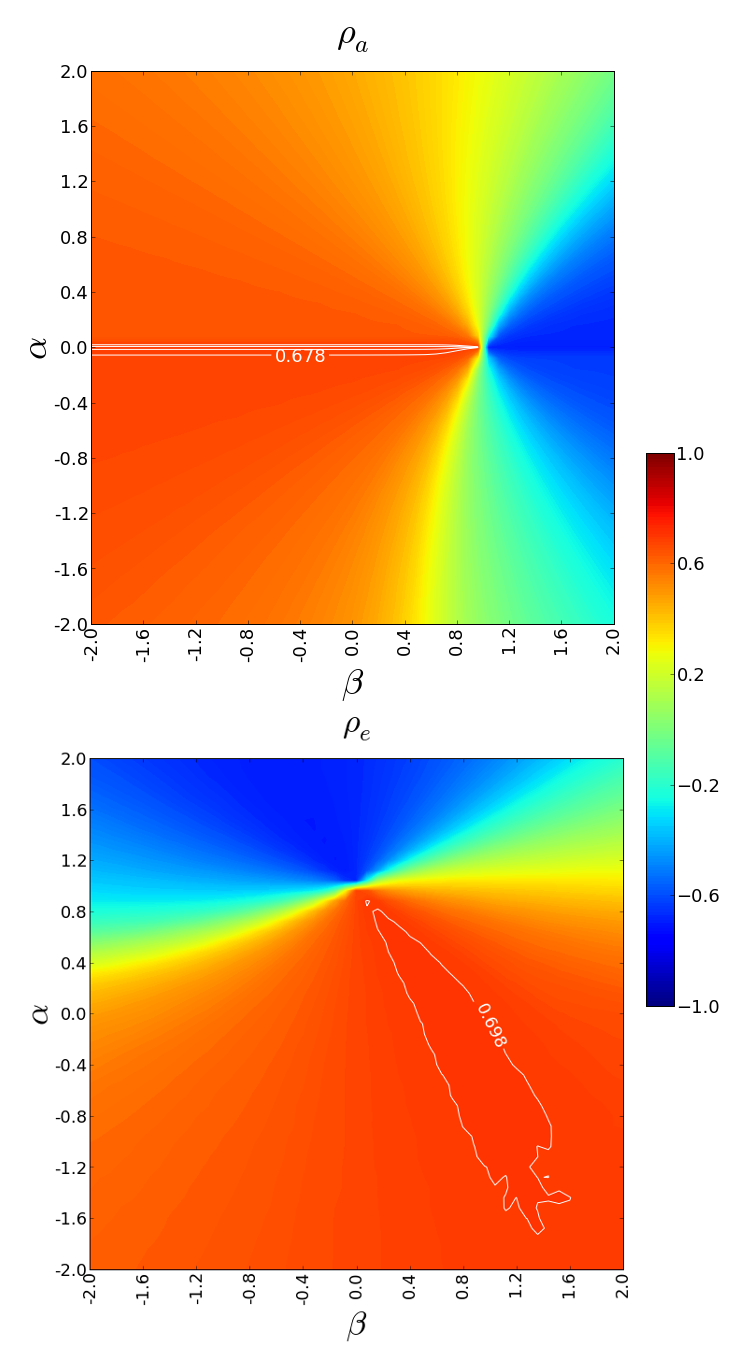
\includegraphics[width=0.9\columnwidth]{../Figures/contour_fem_combined.png}.
\caption{Typical landscape of maximum correlation as a function of $\alpha$ and $\beta$ for articles (upper panel) and editors (lower panel). The contour line shows the 95\textsuperscript{th} percentile of the rank correlation over the landscape. The category displayed here is {\it Feminist Writers}, for the last snapshot ending February 2014.}
\label{fig:landscape}
\end{figure}

The maximum achievable rank-correlation with ground-truth expertise and quality metrics for respectively editors \cite{geiger2013} and articles \cite{wang2013tell} shows that the bi-partite network random walker model accounts particularly well for both quality of articles ($0.58 < \rho_a < 0.91$) and expertise of editors ($0.46 < \rho_e < 0.75 $) at the last snapshot. Actually, the model reproduces very well, and very early the ranking of editors and articles according to the ground-truth metrics as shown on Figure \ref{fig:rhotime}. In particular, the quality of articles is very well accounted for, while the level of correlation with the ground-truth of editor expertise exhibits a slightly concave, or at least linear, increase.

%The question remains if the intersection of the solution spaces for $\rho_a$ and $\rho_e$ is nonempty. That is whether the we can find values of $\alpha$ and $\beta$ for which our editor ranking and article ranking are simultaneously optimized. We exploit two empirical facts from our data: the clear solution for article rankings that $alpha = 0$, and that for editor rankings the 95\textsuperscript{th} percentile maximizing boundary always includes values at $\alpha = 0$. Therefore, with $\alpha = 0$, we solve for $\beta$ in the editor ranking that maximizes $\rho_e$ - and thus $\rho_a$ simultaneously. 

For the latest snapshot (i.e. the state of contributions in February 2014), we find that the best possible $\alpha^*$ is $0$ in all circumstances, while $\beta^*$ varies considerably across categories. Table \ref{tab:maxbeta} shows the categories ordered by $\beta^*$ (and $\alpha^*=0$ for the sake of completeness), as well as the corresponding maximum rank correlations $\rho_e$ and $\rho_a$. Since there is no single optimal value for $(\alpha^*,\beta^*)$, but rather a space of optimal values for  $\rho_e$ and $\rho_a$ separately, we have searched for a set of values that jointly maximizes both $\rho_e$ and $\rho_a$. The optimal parameter $\alpha^* = 0$ means that editor expertise always benefits from contributions as a linear function of the number of articles edited [compounded over iterations of the recursive algorithm defined by formula (\ref{random_walker})].  However, $\beta^*$ exhibits a continuum of values between $0$ ({\it Bicycle parts} and {\it US Military History}) and $1.52$ ({\it Sexual Acts}). $\beta$ controls the influence of the number of editors on the quality of a given article. When $\beta \approx 0$, the quality of articles increases as a linear function of the number of editors who have modified them. For $\beta \gg 0$, the marginal gain of having more editors for a given article decreases. So, in that case, when the number of editors touching an article increases, the marginal quality improvement decreases.

The evolution of $\beta^{*}$ over snapshots as shown on Figure \ref{fig:rhotime} exhibits large variations for early snapshots corresponding to the early 10\% of overall contributions per category (i.e. the 4\textsuperscript{th} snapshot). While $\beta^{*}$ exhibits a tendency to more stability afterwards, large variations within the range $0$ to $1.5$ can be observed for some categories, suggesting that organization changes, along with the coordination level, can occur as categories further develop. 

%In fact, $\beta$ switches signs only 3 times of the possible 144 measured changes. Although there are not enough $\beta < 0$ to draw a firm conclusion, it is interesting to note that instances of $\beta < 0$ happened in early category history, hence suggesting that the early contributions steps pull more value from the community. 
%The stability of $(\alpha^*,\beta^*)$ confirms that the control parameters of the bi-partite network random walker model describe a robust feature of the structure of value creation in the bi-partite network of editors contributing to articles. This additional result is also a first step towards robust predictions of editor expertise and article quality rankings, given successive inputs to new articles made by editors.


\begin{table}
%\end{table}
\begin{tabular}{|llcccc|}
\hline
         &                     Category & $\rho_a$ & $\rho_e$ & $\alpha^{*}$ & $\beta^{*}$ \\
\hline
 1&                        Bicycle parts  &     0.90 &     0.46 &     0.00 &    0.00 \\
 2&Military history of the US  &     0.58 &     0.70 &     0.00 &    0.00 \\
  3&                Computability theory &     0.77 &     0.56 &     0.00 &    0.32 \\
   4&            American male novelists &     0.67 &     0.75 &     0.00 &    0.40 \\
    5&                        2013 films  &     0.72 &     0.55 &     0.00 &    0.48 \\
     6&                Economic theories  &     0.74 &     0.70 &     0.00 &    0.48 \\
     7&         American women novelists  &     0.63 &     0.75 &     0.00 &    0.64 \\
     8&                 Feminist writers  &     0.70 &     0.69 &     0.00 &    0.72 \\
     9&                             Yoga  &     0.64 &     0.57 &     0.00 &    1.12 \\
     10&      Nobel Peace Prize laureates  &     0.91 &     0.66 &     0.00 &    1.20 \\
      11&        Counterculture festivals  &     0.80 &     0.61 &     0.00 &    1.36 \\
        12&                   Sexual acts  &     0.63 &     0.66 &     0.00 &    1.52 \\
\hline
\end{tabular}
\caption{Categories ordered by increasing $\beta^{*}$ obtained from best rank-correlation $\rho_a$ and  $\rho_e$
 of the {bi-partite network random walker} with the ground truth. As shown on the upper panel of Figure \ref{fig:landscape}, highest rank-correlation is always obtained for $\alpha^{*} = 0$ suggesting that editors are experts in direct proportion to the number of articles they edit. The different values of $\beta^{*}$ show the effect of marginal editors on a article. As $\beta^{*}$ grows larger having more editors shows diminishing returns on article quality - ``too many cooks spoil the broth".}
\label{tab:maxbeta}
\end{table}


%However, for categories with $\beta >0$ the quality of an article is also negatively influenced by the portfolio size of its editors. In other words, when $\beta$ is large, the more articles an editor edits, the lower his or her contributed value to one single article. $\beta$ also characterizes each category and the way quality is achieved through the cumulative contribution of information. For $\beta$ small, all editors have a fairly equal chance to contribute positively to any article, while for $\beta$ large, an editor can only contribute positively to a subset of articles (the larger $\beta$ the smaller the set). Typically, it is unlikely for a single person to have visited all {\it counterculture festivals}, performed all {\it sexual acts} or {\it Yoga} practices, while it is easier for anyone to gather relevant information on {\it bicycle parts} or the {\it US military history}. 





%\textcolor{red}{\bf Is there any reshuffling of ranking over time, or do they stay the same?}



\begin{figure}[!t]
\centering
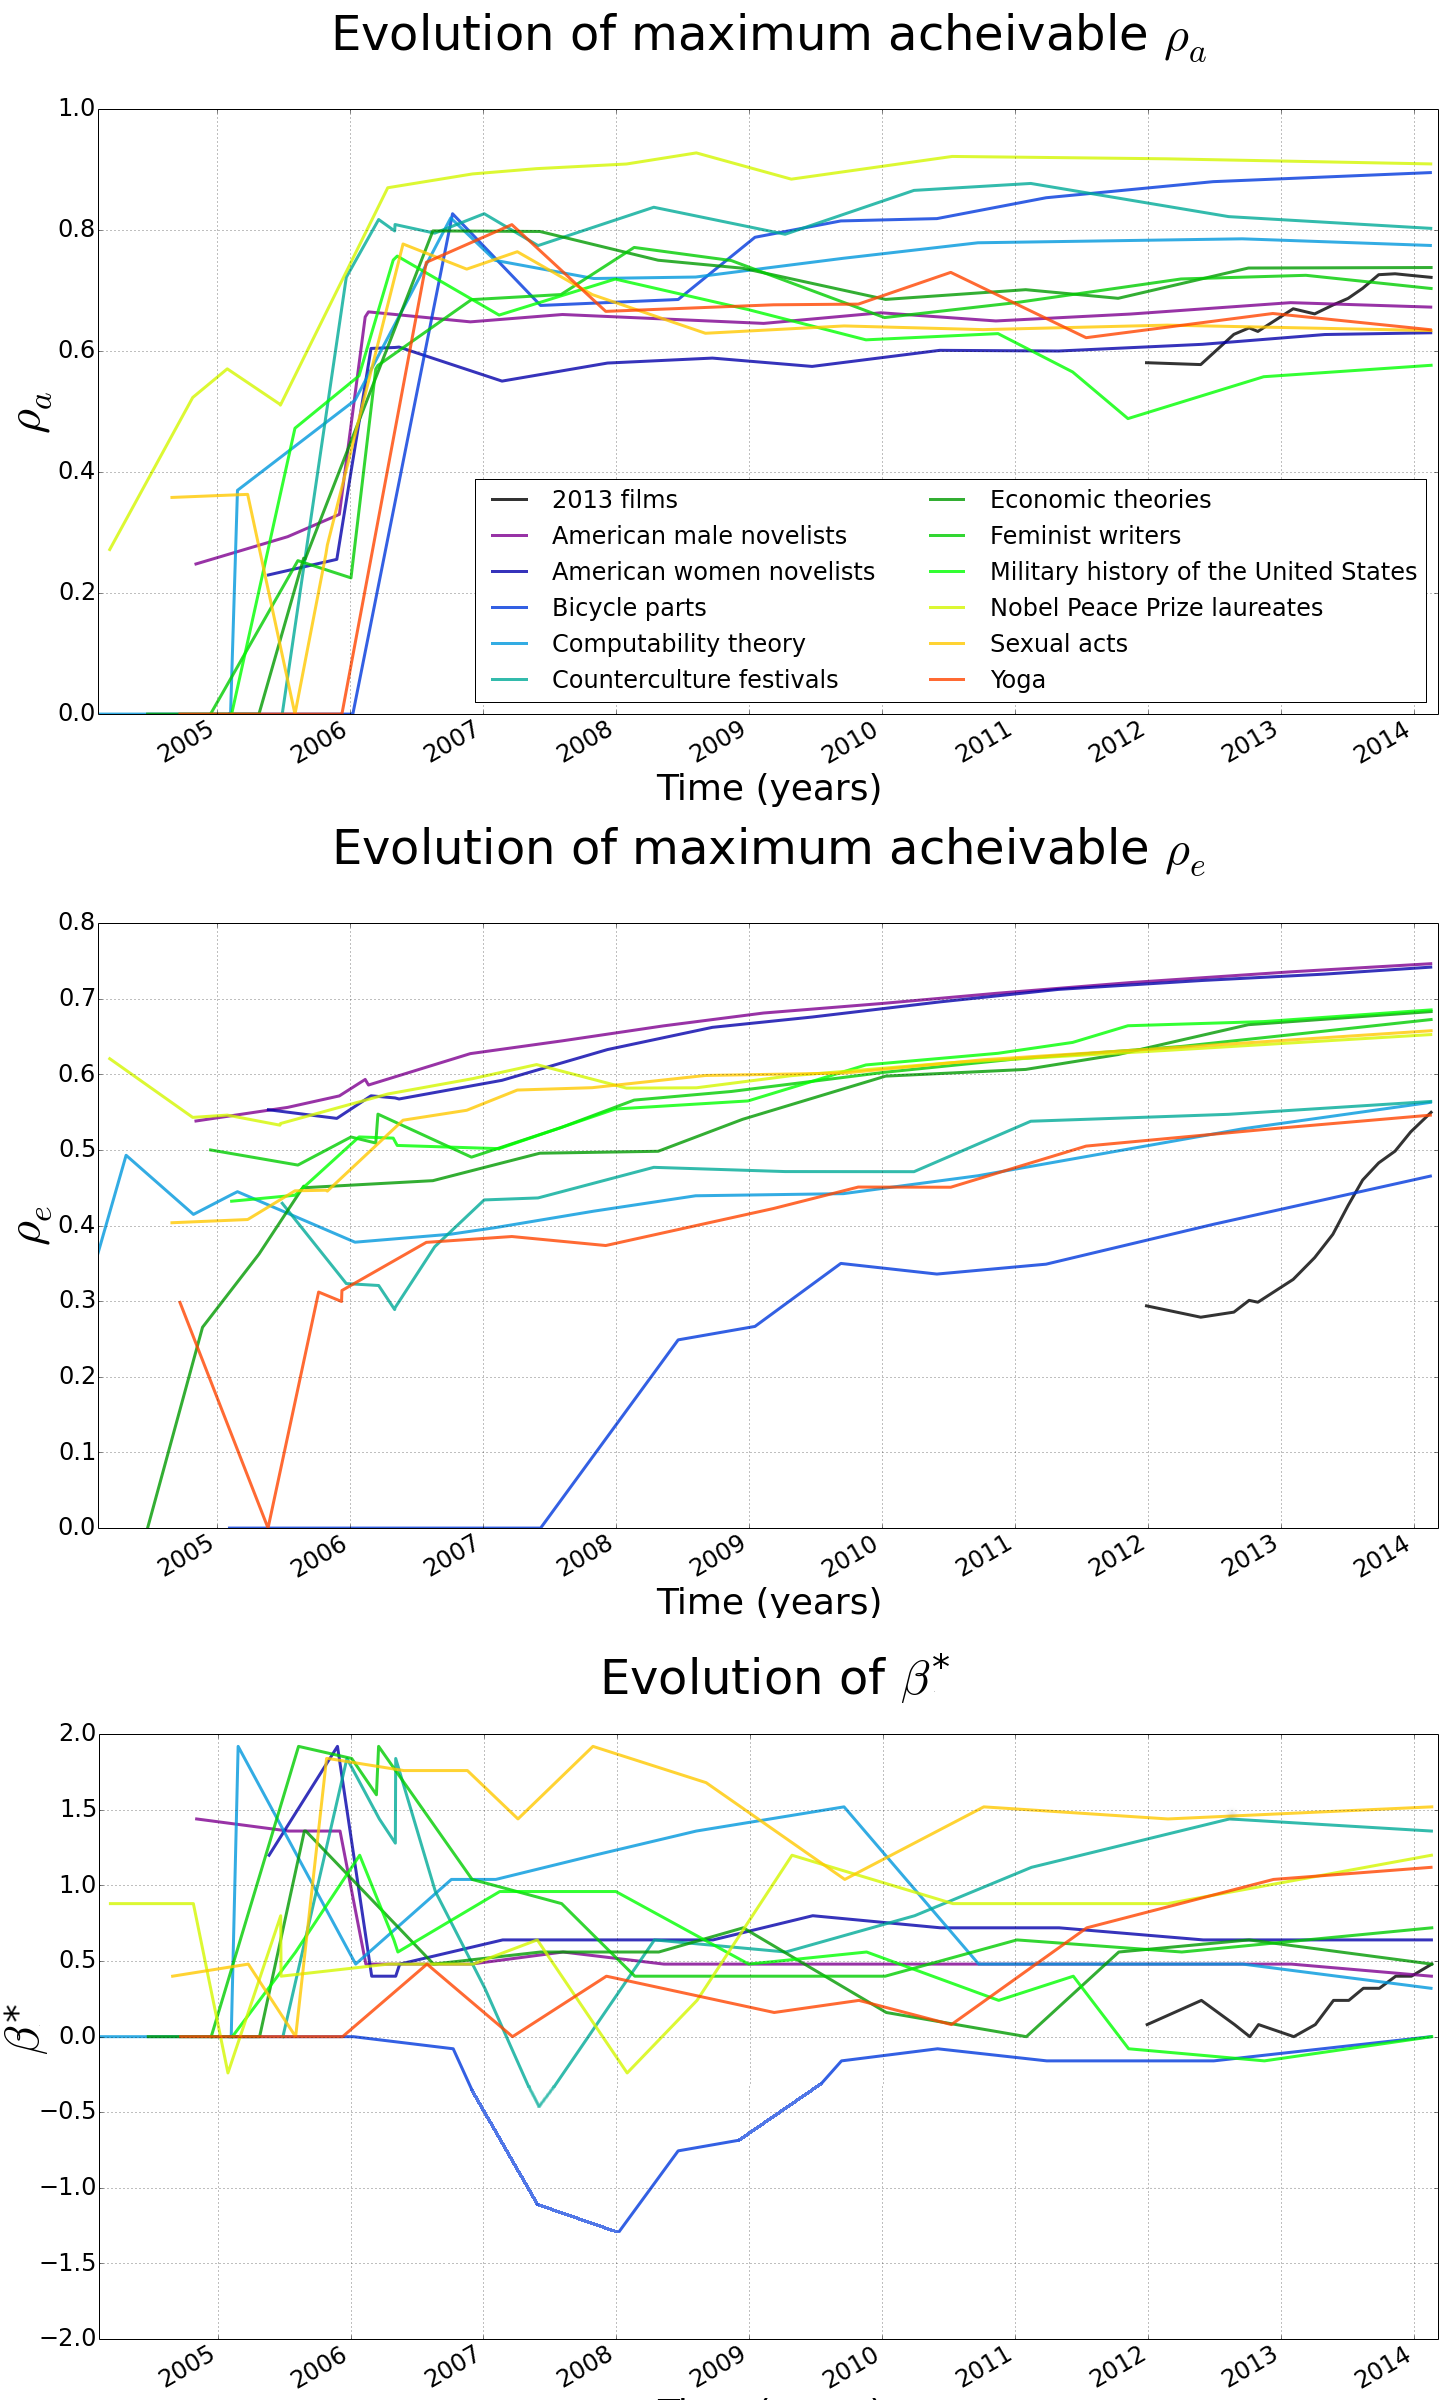
\includegraphics[width=0.9\columnwidth]{../Figures/rho_combined_with_beta.eps}.
\caption{Evolution of Spearman $\rho$ rank correlations between the ranking obtained from the calibrated model and the actual values for each category and for editors (upper panel)  and articles (middle panel). Corresponding $\beta^{*}$ values are also shown for interest (lower panel). The correlations are generally quite high : $ 0.46 < \rho_e < 0.75$ with $\langle \rho_e\rangle = 0.64$ for editors and $0.57 < \rho_a < 0.91$ with $\langle \rho_a\rangle = 0.72$. $\rho_{a}$  is stable over time, which means that the quality of articles can be well captured early on by the model. However, $\rho_e$ exhibits a convex increase over time, suggesting that it takes time (i.e. lots of edits) to capture well the expertise of editors.}
\label{fig:rhotime}


\end{figure}

	



